\chapter{Event Reconstruction and Physics Objects}
\label{CHAPTER:EventReconstructionPhysicsObjects}

\glsresetall % Resetting all acronyms

This chapter describes how the \gls{CMS} detector produces physics objects from the information collected at each event. The \glsreset{VBF} Higgs to invisible analysis uses almost all the physics objects produced by the detector and for this uses information from all the experiment sub-detectors. The following sections detail for each of these objects how they are reconstructed and what are the choices made to filter them.

\section{Tracks}

%Status: DONE

Reconstructing the trajectories of charged particles allows us to measure their momentum and determining their charge. This is possible by analysing the hit patterns in the inner tracking system. In \gls{CMS} this reconstruction is made with the \gls{CTF} algorithm \cite{ARTICLE:CMSTrackReconstruction}. The relevant steps for track generation are described below:

\begin{itemize}
  \item Seed generation is made with hits at the pixel detector. A track seeds can be made with two or three hits. In the first case a know vertex or the beam spot is used to constrain the seed momentum. The parameters of each seed are estimated using the assumption that the trajectory is a helix, but it takes into account hit errors and multiple scattering \cite{ARTICLE:CMSTrackReconstructionSeedGeneration}.
  \item The track seed is extrapolated through the tracker layers with on a combinatorial Kalman filter \cite{ARTICLE:KalmanFilteringTrackVertexFitting} . For each additional layer, the best matching hit if any is added and track parameters are recomputed. This procedure continues until the last layer is reached \cite{ARTICLE:CMSTrackReconstruction}.
  \item Ambiguity resolution may be necessary since since it is possible to have the same track being reconstructed from different seeds, or a seed may results in more than a single trajectory candidate. The resolve this possible double counting, when considering a pair of tracks with more than 50\% of shared hits, we discard the one with less hits. In case so equal number of hits the one with lowest $\chi^2$ is kept. 
  \item After the track building and cleaning stage is done final refitting is performed. This procedure is aimed at removing possible bias by constrains at the seed forming stage. A standard Kalman filter and smoother are used.
\end{itemize}

The process of track finding is repeated up to six times where the hits for each successfully reconstructed track are removed for the next iteration. Using early \gls{LHC} data and a dataset of pions and muons it was possible to estimate that the tracking efficiency is $>98\%$ for all track $\pt > 500\,\MeV$ and $>99\%$ for tracks with $\pt > 2,\GeV$ \cite{ARTICLE:CMSMeasurmentTrackEfficiency}.

\section{Vertex Reconstruction}

%Status: DONE

The \gls{LHC} can produce extreme collision intensities which are obtained partially by having multiple collisions happening at each bunch crossing. As it has been discussed in section \ref{SUBSECTION:ExperimentalApparatus_CMS_RunningAndPerformance} an average of 21 simultaneous collisions happened per bunch crossing in the \gls{CMS} experiment during 2012. In this environment, it is crucial to identify the \gls{PV} and the particles that come from it. This information can then be used to reject particles coming from other additional collisions and to identify displaced vertices which can be the signature of long lived particles like b-mesons.

The individual tracks are reconstructed making use of the inner tracker. Each vertex is initially seeded by two tracks with separation in \textit{z} less than $1\,\centi\meter$. Then remaining track are clustered to seed vertex with the \gls{DA} algorithm \cite{ARTICLE:DeterministicAnnealing}. After the clustering process is done, the position of each vertex is recomputed using the adaptive vertex fitter algorithm \cite{ARTICLE:AdaptiveVertexFitting}. In this algorithm weights, $w_{i}$ are assigned to each track according to how compatible they are with the fitted vertex position. Weight vary from 1 to 0, being that track assigned weights of close 1 are highly compatible with the vertex and close 0 would be given to low compatibility tracks. Then we can define the number of degrees of freedom of the new fit as:

\begin{equation}
n_{dof}(vertex)=2\sum\limits_{i}^{tracks} w_i - 3
\end{equation}

This variable can be used to distinguish real proton-proton interactions from misclustered vertices, since it is correlated with the number of tracks compatible with that specific vertex \cite{ARTICLE:CMSTrackingAndPrimaryVertex}. The vertex position and resolution have been measured with \gls{LHC} data and compared with simulation. The resulting plots can be found in figure \ref{FIGURE:EventReconstructionPhysicsObjects_Vertex} as a function of number of tracks.

\begin{figure}[htp]%
\centering
\subfloat[][]{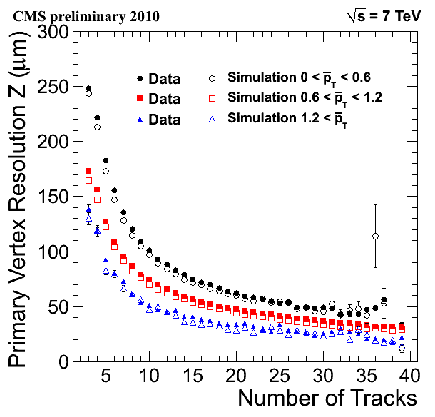
\includegraphics[width=0.45\linewidth]{Chapter04/Vertex/Images/vtx-res.pdf}}\qquad
\subfloat[][]{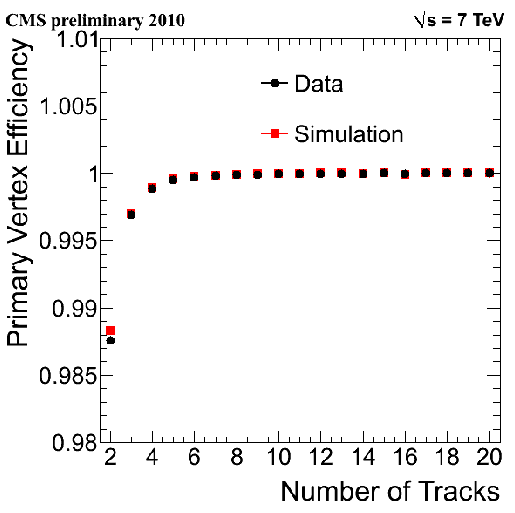
\includegraphics[width=0.45\linewidth]{Chapter04/Vertex/Images/vtx-eff.pdf}}\\
\caption[Primary vertex resolution in the $z$ coordinate and vertex reconstruction efficiency as a function of the number of constituent tracks.]{(a) Primary vertex resolution in the $z$ coordinate a function of the number of associated tracks. Results are give for three ranges of average track \pt. (b) Primary vertex efficiency as a function of the number of associated track \cite{ARTICLE:CMSTrackingAndPrimaryVertex}}
\label{FIGURE:EventReconstructionPhysicsObjects_Vertex}
\end{figure}

The \gls{PV} is defined as the vertex with highest sum of associated tracks \pt squared. In situations were no vertex can be reconstructed, like if there is a tracking failure, the beam spot position is assumed. Knowing precisely the interaction point allows to determine particle candidate quantities relative to it which allow for better object identification and pile-up control. 

Most \gls{CMS} analysis, including the ones presented in this thesis, require explicitly that a good vertex is reconstructed with the following characteristics:

\begin{itemize}
  \item We require a real reconstructed vertex from tracks, not the beam spot.
  \item A minimum number of degrees of freedom: $n_{dof}>4$.
  \item Collision must be near the interaction point. We require longitudinal distance to be $|z|<=24\,\centi\meter$.
  \item We required the collision be be close to the beam line. Radial distance to beam line: $d_{xy}<2\,\centi\meter$. 
\end{itemize}

\section{Electron}

%Status: DONE

In the \gls{CMS} experiment electrons are reconstructed by matching energy clusters in the \gls{ECAL} with tracks coming from the inner tracking system. Unfortunately, electrons can loose and disperse significant amounts of energy until they reach the \gls{ECAL}. While they transverse the inner tracker they may emit photons through bremsstrahlung and in turn this photon can convert to $e^+e^-$ pairs. About 35\% of the electron radiate at least 70\% of their energy in this way \cite{ARTICLE:CMSElectronReconstruction}. This spread of energy is mostly in $\phi$ due to the applied magnetic field \cite{ARTICLE:CMSElectronReconstructionECAL}. Dedicated algorithms were developed to combine the the \gls{ECAL} energy deposits, into a so called \textit{super-clustering algorithm}, of the initial electron and its emissions.

Different algorithms are used in the barrel and endcaps regions. In the barrel region we explore the simple $\eta-\phi$ geometry with the ``hybrid clustering algorithm''. The procedure started by identifying \textit{seed crystals} with $E_\perp>1\,\GeV$. We form a domino around this seed in the $\eta$ direction of $3 \times 1$ or $5 \times 1$ crystals centred at the seed. Additional dominoes are added in both $\phi$ direction in an attempt to collect the bremsstrahlung emissions up to $\Delta\phi \approx 0.3\,\radian$. Any domino with energy below $100\,\MeV$ is disregarded. The resulting additional sub-clusters must have its own seed with $E_\perp>350\,\MeV$ and they are all combined to form the final \textit{supercluster}. 

In the encaps the ``$\text{Multi-}5 \times 5$'' is used. In the region of the detector the geometry is more complex and does not follow a simple $\eta-\phi$ symmetry. We start by selecting for seeds the crystals which are local maxima over their four direct neighbours and have a deposit of $E_\perp>0.18\,\GeV$. Then, and starting with the seeds with highest $E_\perp$, we collect the energy around them into clusters of $5 \times 5$ crystals. We then search for similar seeds and form clusters that can overlap within $\Delta\eta<0.07$ and $\Delta\phi<0.3\,\radian$ of the initial seed. Those clusters are then combined into a single \textit{supercluster} which needs to have at least $E_\perp>1\,\GeV$. The \textit{supercluster} is then extrapolated to the \gls{ECAL} preshower
by clustering the energy within $\Delta\eta<0.15$ and $\Delta\phi<0.45$ around the most energetic cluster and adding it to the \textit{supercluster} itself \cite{ARTICLE:CMSElectronReconstruction8TeV}.

In order to reconstruct the electron track we need to take into account the bremsstrahlung emissions. The \gls{CTF} algorithm is not appropriate for this purpose so a different track-finding algorithm had to be developed. For high \pt electrons we use the \gls{ECAL} supercluster energy deposit weighted mean impact point as a seed. If we combine this information with the determined $E_\perp$ we can define two $\eta-\phi$ search regions in the pixel detector depending on the charge hypothesis. If we find two compatible hits, the electron trajectory is updated. From this point normal track building is performed but instead of a Kalman filter algorithm we use a \gls{GSF} algorithm \cite{ARTICLE:CMSReconstructionElectronsGSF}. This method performs better in the presence of non-Gaussian losses like the one coming from the bremsstrahlung emissions.

The typical background to real electrons are collimated hadronic jets, like from $\pi^0$ and $\pi^{\pm}$ overlap or from $\pi^{\pm}$ showers \cite{ARTICLE:CMSElectronReconstruction}. There are many useful variables that may be used to reduce such background and are often used in \textit{electron identification} criteria:

\begin{itemize}
  \item $\Delta\eta_{in}$ and $\Delta\phi_{in}$, are the distance between the track direction at the vertex and extrapolated to the \gls{ECAL} and supercluster.
  \item $\sigma_{i \eta i \eta}$ is the energy-weighted $\eta$ width of the cluster. For real prompt electrons this is normally small since this quantity is not significantly affected by the magnetic field.
  \item $H/E$ is the ration of hadronic to electromagnetic energy in the region of the seed cluster. 
\end{itemize}

Distributions of the variables for simulated electrons and jets can be found in figure \ref{FIGURE:EventReconstructionPhysicsObjects_Electrons}. 

\begin{figure}[htp]%
\centering
\subfloat[]{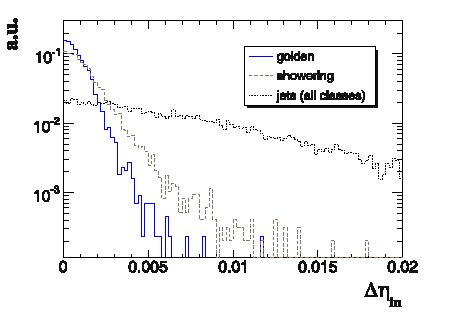
\includegraphics[width=0.45\linewidth]{Chapter04/Electrons/Images/elecs_deta.pdf}}\qquad
\subfloat[]{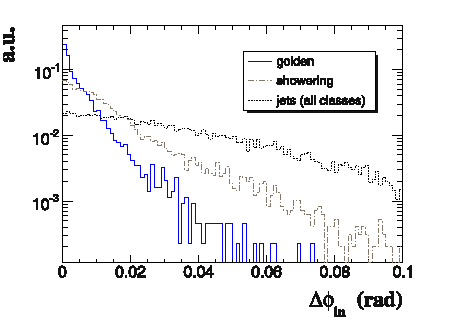
\includegraphics[width=0.45\linewidth]{Chapter04/Electrons/Images/elecs_dphi.pdf}}\\
\subfloat[]{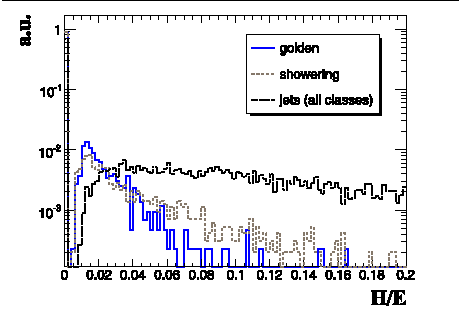
\includegraphics[width=0.45\linewidth]{Chapter04/Electrons/Images/elecs_hovere.pdf}}\qquad
\subfloat[]{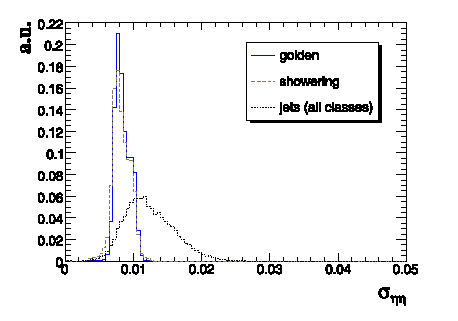
\includegraphics[width=0.45\linewidth]{Chapter04/Electrons/Images/elecs_sigmaietaieta.pdf}}
\caption[Distributions for the variables $\Delta\eta_{\text in}$, $\Delta\phi_{\text in}$, $\sigma_{i\eta i\eta}$ and $H/E$ for simulated electrons and misidentified jets.]{Distributions for (a) $\Delta\eta_{in}$, (b) $\Delta\phi_{in}$, (c) $H/E$ and (d) $\sigma_{i \eta i \eta}$. Here \textit{golden electrons} are those who emit minimal bremmstrahlung photons, \textit{showering} are electrons that lose a large faction of their energy in emissions and \textit{jets} are the typical distributions for hadronic jets.}
\label{FIGURE:EventReconstructionPhysicsObjects_Electrons}
\end{figure}

\section{Muon}

%Status: Writing

Muon track reconstruction starts independently at the inner-tracker (\textit{tracker track} and in the muon systems (\textit{standalone-muon track}) \cite{ARTICLE:CMSMuonReconstruction7TeV}. Then this information can be combined into a single muon track in two possible ways.

\textit{Global Muon reconstruction} is an \textit{outside-in algorithm}. We starts by finding tracker track match for each stand-alone muon track. This is done by propagating the match candidate pair to a common surface and comparing track parameters. For each matched pair, a \textit{global-muon fit} is performed using all hits from the two tracks using a a Kalman-filter algorithm \cite{ARTICLE:KalmanFilteringTrackVertexFitting}. For muons of $\pt\gtrsim 200\,\GeV/c$, it has been showed that a \textit{global-muon fit} improves the momentum resolution compared to a \textit{tracker-only fit} \cite{CMSTDR:CMSPhysicsVol1, ARTICLE:CMSPerformanceMuonReconstructionCosmicRay}.

\textit{Tracker Muon reconstruction} is an \textit{inside-out algorithm}. 


%\cite{ARTICLE:CMSMuonReconstruction7TeV} %AG 72

\section{Particle Flow}

%Status: Writing

\gls{PF}

\cite{ARTICLE:CMSComissioningOfParticleFlow}

\cite{ARTICLE:CMSParticleFlowEventRecontruction}

\cite{ARTICLE:CMSComissioningOfParticleFlowWithMinBias}

\section{Jets}

%Status: Writing

\subsection{Jet Clustering}

\cite{ARTICLE:TowardsJetography}

\cite{ARTICLE:AntiKtAlgorithm}

\cite{ARTICLE:FastJetUserManual}

\subsection{Jet Energy Corrections}

\cite{ARTICLE:CMSDeterminationJetEnergyCalibration}

\cite{ARTICLE:PileupSubtractionJetAreas}

\section{Taus}

\section{Missing Transverse Energy}

\cite{ARTICLE:CMSMissingTransverseEnergyPerformance}

\cite{ARTICLE:CMSMETPerformance8TeV}

